% AICAS 2026 -- 4+1 pages, double-blind, IEEE conference format
% Compile: pdflatex main && bibtex main && pdflatex main && pdflatex main
\documentclass[conference]{IEEEtran}

\usepackage[utf8]{inputenc}
\usepackage[T1]{fontenc}
\usepackage{amsmath,amssymb}
\usepackage{graphicx}
\usepackage{booktabs}
\usepackage{hyperref}
\usepackage{xcolor}
\usepackage{multirow}
\usepackage{array}
\usepackage{url}
\usepackage{balance}
\usepackage{tikz}
\usepackage{pgfplots}
\pgfplotsset{compat=1.18}
\usetikzlibrary{arrows.meta, positioning}
\usepackage{cite}
\usepackage{pifont}

\hypersetup{colorlinks=false}

% Tighter lists
\usepackage{enumitem}
\setlist[itemize]{itemsep=1pt, parsep=0pt, topsep=3pt}

\title{Sub-Millijoule Intrusion Detection on a\\Commodity MCU Neural Processing Unit}

\author{\IEEEauthorblockN{Anonymous}
\IEEEauthorblockA{Double-blind review}}

\begin{document}
\maketitle

% ============================================================
\begin{abstract}
We deploy an intrusion detection system (IDS) classifier on the
STM32N6570-DK, a commodity ARM Cortex-M55 MCU with the Neural-ART NPU
rated at 600\,GOPS INT8.
Exploiting the approximate equivalence between single-timestep
($T{=}1$) spiking neural network (SNN) inference and INT8 quantized
ANN inference, we compile a lightweight MLP to the NPU without
neuromorphic hardware.
On NSL-KDD (5-class) and UNSW-NB15 (10-class) with 10
random seeds, the model achieves $78.86{\pm}1.32$\% and
$64.75{\pm}0.61$\% overall accuracy, respectively.
INT8 NPU inference completes in \textbf{0.29--0.46\,ms}
(2.7--4.2$\times$ faster than CPU-only), with an estimated energy
of \textbf{44--69\,\textmu J/inference} and a Flash footprint of
120--138\,KB.
Compared with recent MCU-class IDS deployments on the STM32F7
(31\,ms, 7.86\,mJ) and Raspberry Pi~3 (27\,ms), our NPU path
achieves 60--107$\times$ lower latency and over 100$\times$
lower energy per inference.
To our knowledge, this is the first publicly documented IDS
deployment on an ARM Cortex-M NPU, and also the first non-vision
workload reported on the Neural-ART accelerator.
\end{abstract}

\begin{IEEEkeywords}
intrusion detection, spiking neural network, neural processing unit,
INT8 quantization, edge AI, STM32N6
\end{IEEEkeywords}

% ============================================================
\section{Introduction}
\label{sec:intro}

Deep-learning-based intrusion detection at the IoT edge must operate
under tight power and latency budgets.
Recent MCU-class deployments achieve promising accuracy but at high
energy cost: Chehade et~al.\ reported 31\,ms and 7.86\,mJ per
inference on an STM32F746G (Cortex-M7, no NPU)~\cite{chehade2025stm32},
and Diab et~al.\ required 27\,ms on a Raspberry~Pi~3B+~\cite{diab2025rpi}.
At these latencies, CPU-only inference blocks all concurrent RTOS tasks
for tens of milliseconds, making real-time packet processing difficult.

Commodity MCUs are beginning to integrate neural processing units (NPUs)
that execute INT8 matrix operations at hundreds of GOPS while freeing
the CPU for other tasks.
A line of theoretical work~\cite{bu2022optimal, jiang2023unified,
bu2025inference} has shown that single-timestep ($T{=}1$) SNN inference
is approximately equivalent to INT8 quantized ANN inference:
when the membrane potential is initialized to zero, the
threshold-and-fire mechanism reduces to a ReLU-like clamp.
Any NPU executing INT8 \texttt{Gemm}+\texttt{Relu} can therefore
run an SNN-equivalent model.

We validate this on the STM32N6570-DK (ARM Cortex-M55
@ 800\,MHz, Neural-ART NPU, 600\,GOPS INT8, \$89 dev kit).
We focus on classifier inference latency, energy, and memory footprint
on pre-extracted flow-level features; the full IDS pipeline (packet
capture, flow aggregation) is left to future work.

Our contributions:
\begin{itemize}
  \item To our knowledge, the first publicly documented IDS classifier
    deployment on an ARM Cortex-M NPU,
    achieving 0.29--0.46\,ms inference at an estimated 44--69\,\textmu J.
  \item Empirical validation of $T{=}1$ SNN--ANN equivalence on
    commercial NPU silicon, with 99\% prediction agreement between
    FP32 and INT8 models.
  \item An operator-level analysis showing that the \texttt{Floor}
    operator required by QCFS~\cite{bu2022optimal} falls back to CPU,
    adding 17.6\% latency.
\end{itemize}

% ============================================================
\section{Related Work}
\label{sec:related}

Table~\ref{tab:related} compares IDS deployments on physical hardware.
Ngo et~al.~\cite{ngo2022hhnids} deployed a 1,360-parameter MLP on
the MAX78000, an AI-specialized MCU with a fixed CNN accelerator,
achieving 98.57\% on UNSW-NB15 (binary) at 18\,mW.
Zahm et~al.~\cite{zahm2024csiac} used the BrainChip Akida AKD1000
neuromorphic processor (98.4\%, ${\sim}$1\,W).
Both use purpose-built AI/neuromorphic hardware.
Chehade et~al.~\cite{chehade2025stm32} deployed a 1D-CNN on the
STM32F746G (Cortex-M7, no NPU), achieving 96.59\% accuracy on
ISCX VPN-nonVPN but requiring 31\,ms and 7.86\,mJ per inference.
Diab et~al.~\cite{diab2025rpi} deployed LightGBM/CNN on Raspberry~Pi~3B+
(27--300\,ms, 250--275\,mW).
Our work targets a general-purpose MCU with an attached programmable NPU,
achieving two orders of magnitude lower energy than CPU-only MCU
deployments.

Several GPU-based SNN-IDS systems have also been proposed:
convolutional SNNs~\cite{nature2024csnn},
event-driven SNNs~\cite{ieee2025event}, and transformer-spiking
hybrids~\cite{nature2026transformer} report 94--99\% accuracy on
NSL-KDD/UNSW-NB15 but use binary classification and have no path
to edge deployment.
Our multi-class formulation (5/10-class) and hardware deployment
target a different design point.

\begin{table}[t]
\centering
\caption{Hardware-deployed IDS comparison. Energy is per inference.}
\label{tab:related}
\small
\resizebox{\columnwidth}{!}{%
\begin{tabular}{@{}llllrrc@{}}
\toprule
\textbf{Work} & \textbf{Platform} & \textbf{Task} & \textbf{Acc.} & \textbf{Lat.} & \textbf{Energy} & \textbf{NPU} \\
\midrule
Ngo~\cite{ngo2022hhnids} & MAX78000 & bin. & 98.6\% & --- & 18\,mW$^*$ & CNN eng. \\
Zahm~\cite{zahm2024csiac} & Akida & multi & 98.4\% & --- & ${\sim}$1\,W$^*$ & Neurom. \\
Chehade~\cite{chehade2025stm32} & STM32F7 & multi & 96.6\% & 31\,ms & 7.86\,mJ & None \\
Diab~\cite{diab2025rpi} & RPi~3B+ & multi & 95.3\% & 27\,ms & ${\sim}$6.75\,mJ & None \\
\midrule
\textbf{This work} & \textbf{STM32N6} & \textbf{5/10} & \textbf{78.9/64.8\%}$^\dagger$ & \textbf{0.29\,ms} & \textbf{44\,\textmu J} & \textbf{NPU} \\
\bottomrule
\multicolumn{7}{l}{\scriptsize $^*$Power, not energy; latency not reported.} \\
\multicolumn{7}{l}{\scriptsize $^\dagger$NSL-KDD 5-class / UNSW-NB15 10-class.}
\end{tabular}%
}
\end{table}

% ============================================================
\section{System Design}
\label{sec:system}

\subsection{$T{=}1$ SNN--ANN Equivalence}

A Leaky Integrate-and-Fire (LIF) neuron updates its membrane potential
$V[t] = \beta \cdot V[t{-}1] + \mathbf{W}\mathbf{x}[t]$ and fires
when $V[t] > \theta$.
At $T{=}1$ with $V[0]{=}0$, the leak term vanishes and firing reduces
to $\Theta(\mathbf{W}\mathbf{x} - \theta)$, which is equivalent to a
quantized ReLU.
Bu et~al.~\cite{bu2022optimal} formalized this via QCFS;
Jiang et~al.~\cite{jiang2023unified} and
Bu et~al.~\cite{bu2025inference} further showed that INT8
post-training quantization produces a discretization grid that closely
approximates the threshold-and-fire operation.
In practice, any NPU that runs INT8 \texttt{Gemm}+\texttt{Relu}
is executing SNN-equivalent computation.

\subsection{Neural-ART NPU}

The STM32N6570-DK pairs an ARM Cortex-M55 at 800\,MHz with the
Neural-ART NPU rated at 600\,GOPS for INT8 and 3\,TOPS/W
efficiency~\cite{st_neural_art}.
The NPU supports \texttt{Conv}, \texttt{Gemm}, \texttt{Relu},
\texttt{Add}, \texttt{Clip}, and \texttt{MaxPool} in INT8;
unsupported operators fall back to the Cortex-M55 CPU with
automatic cache-maintenance overhead at each NPU$\leftrightarrow$CPU
handoff.
The dev kit costs \$89 and includes 4.2\,MB internal SRAM and
128\,MB external NOR Flash.

\subsection{Model Architecture}

We use a four-layer MLP with BatchNorm and ReLU:
$\texttt{Lin}(d{\to}256) \to \texttt{BN} \to \texttt{ReLU}$
$\to \texttt{Lin}(256{\to}256) \to \texttt{BN} \to \texttt{ReLU}$
$\to \texttt{Lin}(256{\to}128) \to \texttt{BN} \to \texttt{ReLU}$
$\to \texttt{Lin}(128{\to}C)$,
where $d{=}41$ (NSL-KDD) or $34$ (UNSW-NB15) and $C{=}5$ or $10$.
BatchNorm is folded into the preceding Linear at ONNX export, yielding
a graph of \texttt{Gemm}+\texttt{Relu} operators only (110--111K parameters).
The architecture is deliberately shallow: deeper models could improve
minority-class recall but risk introducing operators outside the NPU's
supported set.
All hidden dimensions are powers of two (256, 128), avoiding a known
Neural-ART compiler issue with prime-number channel
counts~\cite{st_neural_art}.

\subsection{Datasets and Training}

\textbf{NSL-KDD}~\cite{tavallaee2009nslkdd}: 125,973 train / 22,544 test,
41 features, 5-class.
\textbf{UNSW-NB15}~\cite{moustafa2015unsw}: 175,341 train / 82,332 test,
34 features, 10-class.
Training: Adam ($\text{lr}{=}10^{-3}$), cosine annealing, 80 epochs,
inverse-frequency class weighting, 10 seeds.
Three categorical features are label-encoded; remaining features are
z-score normalized using training-set statistics.
FP32 models are quantized to INT8 via ONNX Runtime static PTQ
(MinMax, per-tensor, 1,000 calibration samples).
A 24-configuration ablation (Section~\ref{sec:quant}) confirms that
the choice of calibration method, granularity, and sample size
changes accuracy by at most 0.82\,pp.

\subsection{NPU Compilation and Operator Mapping}

Models are compiled for the STM32N6570-DK using ST Edge AI Developer
Cloud v4.0.0 (\texttt{atonn} v1.1.3).
Table~\ref{tab:opmap} shows the operator-level mapping.
All \texttt{Gemm}+\texttt{Relu} layers map to NPU hardware epochs.
The \texttt{QuantizeLinear}/\texttt{DequantizeLinear} operators at
the model boundary may require CPU epochs depending on the input
dimension.

\begin{table}[t]
\centering
\caption{Operator mapping to NPU epochs. ReLU INT8 achieves near-100\%
NPU utilization; QCFS INT8 forces CPU fallback at every \texttt{Floor}.}
\label{tab:opmap}
\small
\resizebox{\columnwidth}{!}{%
\begin{tabular}{@{}llcl@{}}
\toprule
\textbf{ONNX Operator} & \textbf{NPU Support} & \textbf{Epoch Type} & \textbf{Notes} \\
\midrule
\texttt{Gemm} (INT8)  & \checkmark & HW & Fused weight + bias \\
\texttt{Relu}          & \checkmark & HW & Fused with preceding Gemm \\
\texttt{Clip}          & \checkmark & HW & Used by QCFS \\
\texttt{Floor}         & \ding{55}  & SW (float) & CPU fallback, +0.08\,ms \\
\texttt{QuantizeLinear}   & \checkmark & HW/Hyb & At model boundary \\
\texttt{DequantizeLinear} & \checkmark & HW/Hyb & At model boundary \\
\bottomrule
\end{tabular}%
}
\end{table}

For the ReLU INT8 path:
NSL-KDD compiles to 5~HW + 1~Hyb + 2~SW epochs (0.46\,ms);
UNSW-NB15 compiles to 4~HW + 0~Hyb + 0~SW epochs (0.29\,ms, 100\% NPU).
The QCFS INT8 path compiles to 13~HW + 1~Hyb + 14~SW epochs (0.54\,ms)
because each \texttt{Floor} triggers a CPU round-trip via
\mbox{\texttt{Dequant}}$\to$\mbox{\texttt{Floor}}$\to$\mbox{\texttt{Quant}}.

% ============================================================
\section{Experiments}
\label{sec:experiments}

\subsection{Classification Results}

\begin{table}[t]
\centering
\caption{Test accuracy (\%, mean$\pm$std, 10 seeds). MLP is the only
model eligible for NPU acceleration.}
\label{tab:accuracy}
\small
\resizebox{\columnwidth}{!}{%
\begin{tabular}{@{}llccc@{}}
\toprule
\textbf{Dataset} & \textbf{Model} & \textbf{Overall} & \textbf{Macro F1} & \textbf{NPU?} \\
\midrule
\multirow{3}{*}{NSL-KDD}
  & ReLU MLP     & \textbf{78.86$\pm$1.32} & \textbf{59.20$\pm$2.80} & \checkmark \\
  & QCFS MLP     & 77.82$\pm$1.11 & 57.29$\pm$2.77 & Partial \\
  & Rand.\ Forest & 73.84$\pm$0.19 & 47.13$\pm$0.33 & \ding{55} \\
\midrule
\multirow{2}{*}{UNSW-NB15}
  & ReLU MLP     & 64.75$\pm$0.61 & 40.29$\pm$0.90 & \checkmark \\
  & Rand.\ Forest & \textbf{69.46$\pm$0.10} & \textbf{48.63$\pm$0.38} & \ding{55} \\
\bottomrule
\end{tabular}%
}
\end{table}

Table~\ref{tab:accuracy} reports multi-seed results.
On NSL-KDD, the ReLU MLP outperforms both QCFS (Wilcoxon $p{=}0.037$)
and tree baselines.
On UNSW-NB15 (10-class), Random Forest achieves higher overall accuracy,
but cannot be compiled for the NPU:
ST Edge AI Core rejects \texttt{TreeEnsembleClassifier} with
``NOT IMPLEMENTED.''
The accuracy gap reflects the difficulty of 10-class classification
with extreme imbalance (Worms: 44 samples), not a modeling limitation
specific to NPU deployment.

Per-class analysis on NSL-KDD reveals that DoS (F1$=$87.3\%) and
Normal (82.6\%) are well-classified, while R2L suffers from low recall
(25.0\%) --- 64.4\% of R2L samples are misclassified as Normal.
U2R (200 test samples) scatters across Probe (50.9\%) and Normal (24.0\%).
On UNSW-NB15, Generic achieves F1$=$97.9\%, but minority classes
collapse: Worms F1$=$9.0\%, Analysis F1$=$2.6\%.
These patterns are characteristic of extreme class imbalance, not
NPU-induced degradation --- FP32 and INT8 models agree on 99\% of
predictions.

Fig.~\ref{fig:cm} visualizes these patterns.
The class imbalance is severe: R2L has only 995 training samples
(0.8\% of the set) yet 2,754 test samples (12.2\%); U2R has 52
training samples.

\begin{figure}[t]
\centering
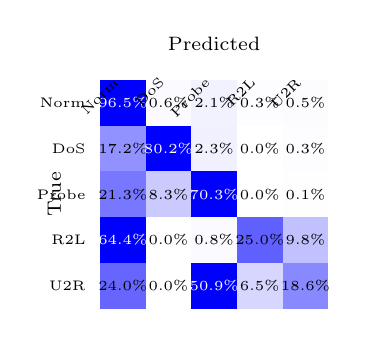
\begin{tikzpicture}[scale=0.58]
% 10-seed mean confusion matrix, verified against multiseed_experiment.json
% Class order: Norm, DoS, Probe, R2L, U2R
% Row 0: Normal
\foreach \x/\v [count=\i from 0] in {96.5/96.5, 0.6/0.6, 2.1/2.1, 0.3/0.3, 0.5/0.5} {
  \pgfmathsetmacro{\c}{min(\x*2.5,100)} \fill[blue!\c!white] (\i,0) rectangle (\i+1,-1);
  \pgfmathtruncatemacro{\w}{\x>50?1:0}
  \ifnum\w=1 \node[font=\tiny,white] at (\i+0.5,-0.5) {\v\%};
  \else \node[font=\tiny] at (\i+0.5,-0.5) {\v\%}; \fi}
% Row 1: DoS
\foreach \x/\v [count=\i from 0] in {17.2/17.2, 80.2/80.2, 2.3/2.3, 0.0/0.0, 0.3/0.3} {
  \pgfmathsetmacro{\c}{min(\x*2.5,100)} \fill[blue!\c!white] (\i,-1) rectangle (\i+1,-2);
  \pgfmathtruncatemacro{\w}{\x>50?1:0}
  \ifnum\w=1 \node[font=\tiny,white] at (\i+0.5,-1.5) {\v\%};
  \else \node[font=\tiny] at (\i+0.5,-1.5) {\v\%}; \fi}
% Row 2: Probe
\foreach \x/\v [count=\i from 0] in {21.3/21.3, 8.3/8.3, 70.3/70.3, 0.0/0.0, 0.1/0.1} {
  \pgfmathsetmacro{\c}{min(\x*2.5,100)} \fill[blue!\c!white] (\i,-2) rectangle (\i+1,-3);
  \pgfmathtruncatemacro{\w}{\x>50?1:0}
  \ifnum\w=1 \node[font=\tiny,white] at (\i+0.5,-2.5) {\v\%};
  \else \node[font=\tiny] at (\i+0.5,-2.5) {\v\%}; \fi}
% Row 3: R2L
\foreach \x/\v [count=\i from 0] in {64.4/64.4, 0.0/0.0, 0.8/0.8, 25.0/25.0, 9.8/9.8} {
  \pgfmathsetmacro{\c}{min(\x*2.5,100)} \fill[blue!\c!white] (\i,-3) rectangle (\i+1,-4);
  \pgfmathtruncatemacro{\w}{\x>50?1:0}
  \ifnum\w=1 \node[font=\tiny,white] at (\i+0.5,-3.5) {\v\%};
  \else \node[font=\tiny] at (\i+0.5,-3.5) {\v\%}; \fi}
% Row 4: U2R
\foreach \x/\v [count=\i from 0] in {24.0/24.0, 0.0/0.0, 50.9/50.9, 6.5/6.5, 18.6/18.6} {
  \pgfmathsetmacro{\c}{min(\x*2.5,100)} \fill[blue!\c!white] (\i,-4) rectangle (\i+1,-5);
  \pgfmathtruncatemacro{\w}{\x>50?1:0}
  \ifnum\w=1 \node[font=\tiny,white] at (\i+0.5,-4.5) {\v\%};
  \else \node[font=\tiny] at (\i+0.5,-4.5) {\v\%}; \fi}
% Labels
\foreach \lab/\y in {Norm/0, DoS/1, Probe/2, R2L/3, U2R/4} {
  \node[font=\tiny, rotate=45, anchor=east] at (\y+0.5, 0.15) {\lab};
  \node[font=\tiny, anchor=east] at (-0.1,-\y-0.5) {\lab};
}
\node[font=\scriptsize, rotate=90] at (-1.0,-2.5) {True};
\node[font=\scriptsize] at (2.5, 0.8) {Predicted};
\end{tikzpicture}
\caption{NSL-KDD confusion matrix (\%, 10-seed mean, ReLU INT8).
R2L$\to$Normal (64.4\%) and U2R$\to$Probe (50.9\%) dominate errors.}
\label{fig:cm}
\end{figure}

\subsection{Energy, Latency, and Memory}

\begin{table}[t]
\centering
\caption{NPU benchmark on STM32N6570-DK. Energy estimated from
AN5946~\cite{st_an5946} (${\sim}$150\,mW at nominal frequency);
FP32 CPU-only power differs and is not estimated (---).}
\label{tab:npu}
\small
\resizebox{\columnwidth}{!}{%
\begin{tabular}{@{}llccccccc@{}}
\toprule
\textbf{Model} & \textbf{Dataset} & \textbf{Time} & \textbf{Energy} & \textbf{HW} & \textbf{Hyb} & \textbf{SW} & \textbf{Flash} & \textbf{RAM} \\
 & & \textbf{(ms)} & \textbf{(\textmu J)} & & & & \textbf{(KB)} & \textbf{(KB)} \\
\midrule
ReLU FP32 & NSL-KDD & 1.24 & --- & 0 & 0 & 11 & 466.4 & 2.17 \\
ReLU INT8 & NSL-KDD & 0.46 & 69 & 5 & 1 & 2 & 137.7 & 1.25 \\
\midrule
ReLU FP32 & UNSW-NB15 & 1.23 & --- & 0 & 0 & 11 & 461.9 & 2.14 \\
ReLU INT8 & UNSW-NB15 & \textbf{0.29} & \textbf{44} & 4 & 0 & 0 & 120.6 & 0.50 \\
\midrule
QCFS INT8 & NSL-KDD & 0.54 & 81 & 13 & 1 & 14 & 138.0 & 2.00 \\
\bottomrule
\end{tabular}%
}
\end{table}

Table~\ref{tab:npu} presents benchmark results from ST Edge AI
Developer Cloud, which cycle-accurately simulates the STM32N6570-DK.
INT8 NPU execution yields \textbf{2.7$\times$} speedup on NSL-KDD
and \textbf{4.2$\times$} on UNSW-NB15 over the same model on
the Cortex-M55 CPU.
At an estimated 150\,mW (ST AN5946~\cite{st_an5946}), this translates
to 44--69\,\textmu J per inference ---
\textbf{over 100$\times$} less than Chehade et~al.'s 7.86\,mJ on
the STM32F7~\cite{chehade2025stm32}.
UNSW-NB15 achieves 100\% NPU execution (4~HW, 0~SW epochs);
Flash shrinks 3.4--3.8$\times$ from FP32 to INT8.

The energy figure is derived from the reference workload in AN5946,
not direct measurement of our model. On-board validation with an
STLINK-V3PWR probe is left to future work.

\subsection{INT8 Quantization Robustness}
\label{sec:quant}

\begin{figure}[t]
\centering
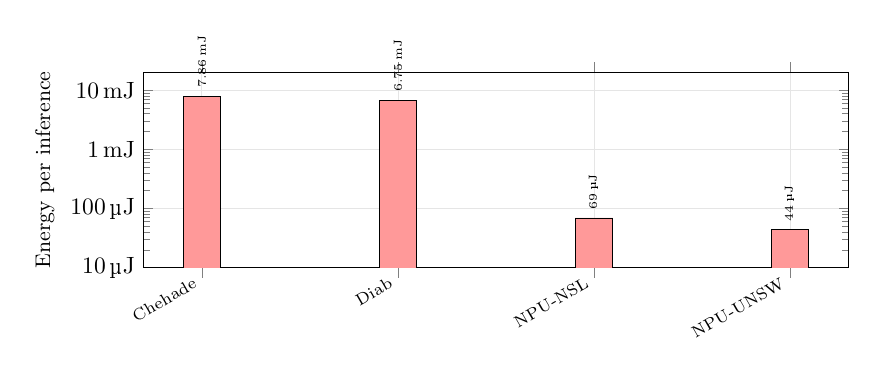
\begin{tikzpicture}[scale=0.85]
\begin{axis}[
    ybar,
    bar width=16pt,
    ylabel={Energy per inference},
    ylabel style={font=\small},
    symbolic x coords={Chehade,Diab,NPU-NSL,NPU-UNSW},
    xtick=data,
    x tick label style={rotate=30, anchor=east, font=\scriptsize},
    ymode=log,
    ymin=10,
    ymax=20000,
    ytick={10,100,1000,10000},
    yticklabels={10\,\textmu J,100\,\textmu J,1\,mJ,10\,mJ},
    ytick style={font=\scriptsize},
    nodes near coords,
    every node near coord/.append style={font=\tiny, rotate=90, anchor=west},
    point meta=explicit symbolic,
    width=\columnwidth,
    height=4.5cm,
    grid=major,
    grid style={gray!20},
]
\addplot[fill=red!40] coordinates {
    (Chehade,7860) [7.86\,mJ]
    (Diab,6750) [6.75\,mJ]
    (NPU-NSL,69) [69\,\textmu J]
    (NPU-UNSW,44) [44\,\textmu J]
};
\end{axis}
\end{tikzpicture}
\caption{Energy per inference (log scale). Our NPU path achieves
over 100$\times$ reduction versus prior MCU-class deployments.
NPU = ReLU INT8 on Neural-ART (estimated from AN5946).
Chehade~\cite{chehade2025stm32}: STM32F7;
Diab~\cite{diab2025rpi}: RPi~3B+.}
\label{fig:energy}
\end{figure}

A 24-configuration ablation (3 calibration methods $\times$
2 granularities $\times$ 4 sample sizes) shows that INT8 accuracy
deviates from FP32 by at most 0.82\,pp across all configurations.
Several INT8 configurations slightly \emph{improve} over FP32,
likely due to regularization effects of quantization noise.

Table~\ref{tab:layerwise} presents layer-wise activation comparison
between FP32 and INT8 models on 1,000 NSL-KDD test samples.
Hidden layers show moderate cosine similarity (0.65--0.68) due to
per-neuron quantization noise, but the logit layer recovers to 0.978
and the overall prediction agreement is 99.0\%.
INT8 maps each activation to one of 256 discrete levels; the bounded
per-neuron noise does not propagate into classification errors.
From the $T{=}1$ SNN perspective, the quantized model (INT8) closely
reproduces the firing decisions of the FP32 model.

\begin{table}[t]
\centering
\caption{Layer-wise FP32 vs INT8 comparison (1,000 NSL-KDD samples).}
\label{tab:layerwise}
\small
\begin{tabular}{@{}lccc@{}}
\toprule
\textbf{Layer} & \textbf{Cosine Sim} & \textbf{MAE} & \textbf{$L_\infty$} \\
\midrule
Relu\_0 (256) & 0.667 & 0.435 & 43.7 \\
Relu\_1 (256) & 0.655 & 0.438 & 62.6 \\
Relu\_2 (128) & 0.683 & 0.400 & 65.2 \\
Logits (5)    & \textbf{0.978} & 0.103 & 19.8 \\
\bottomrule
\end{tabular}
\end{table}

% ============================================================
\section{Discussion and Conclusion}
\label{sec:conclusion}

\textbf{Design-space positioning.}
This work targets a different point from GPU-based IDS: sub-millisecond,
sub-millijoule inference on a \$89 MCU.
The absolute accuracy (78.9\% NSL-KDD, 64.8\% UNSW-NB15) is below
GPU-simulation results, reflecting multi-class evaluation
(5/10-class vs.\ binary) and NPU operator constraints (shallow MLP).
Improving accuracy within these constraints is orthogonal to the
deployment findings.

\textbf{Why NPU over CPU?}
NPU inference frees the Cortex-M55 for RTOS tasks (packet capture,
feature extraction), whereas CPU-only inference blocks the processor
for 1.2\,ms.
Tree models achieve higher accuracy on UNSW-NB15 but have no
execution path on the NPU (\texttt{TreeEnsembleClassifier} is
not implemented in ST Edge AI Core).

\textbf{QCFS barrier.}
The \texttt{Floor} operator is absent from the Neural-ART operator set,
forcing CPU fallback with 17.6\% latency overhead.
ReLU INT8 remains the optimal activation for commodity MCU NPUs.

\textbf{RTOS implications.}
At 0.29--0.46\,ms, NPU inference fits within a typical 1\,ms RTOS
tick, and the Cortex-M55 remains free for concurrent tasks
(Ethernet DMA, feature extraction) during NPU execution.
The 1.2\,ms CPU-only path would block the processor across
tick boundaries. Validating this with \textmu T-Kernel~3.0 is
planned future work.

\textbf{Limitations.}
We measure latency via ST Cloud benchmark; energy is estimated from
the AN5946 application note, not direct measurement of our model.
The evaluation covers classifier inference on pre-extracted features,
not the complete IDS pipeline.
NSL-KDD is a legacy dataset, and UNSW-NB15 has extreme class
imbalance that limits absolute accuracy.

\textbf{Conclusion.}
We demonstrated sub-millisecond, sub-millijoule IDS inference on a
commodity MCU NPU, achieving 2.7--4.2$\times$ CPU speedup and over
100$\times$ energy reduction versus prior MCU-class deployments.
Layer-wise analysis confirms 99\% FP32/INT8 prediction agreement,
validating $T{=}1$ SNN--ANN equivalence on commercial NPU silicon.
Code and trained models will be released upon acceptance.

% ============================================================
\balance
\clearpage
{\small
\bibliographystyle{IEEEtran}
\bibliography{references}
}

\end{document}
